\documentclass[conference]{IEEEtran}
\usepackage[utf8]{inputenc}
\usepackage{textcomp}
\usepackage[spanish]{babel}
\usepackage{amsmath}
\usepackage{amsfonts}
\usepackage{amssymb}
%Dependencies for [1.]
\usepackage{enumerate}
%Dependencies for [1.]
\usepackage{graphicx}
%\usepackage{xcolor}
% Dependencies for Excel2Latex
\usepackage[table]{xcolor}
\usepackage{booktabs}
% Dependencies for Excel2Latex
\usepackage{listings}
\usepackage{tikz}
\usepackage{float}
\usepackage{karnaugh-map}
\usepackage{adjustbox}
\usepackage[left=1cm,right=1cm,top=1cm,bottom=1cm]{geometry}

%Habilita bookmarks en PDF
\newcommand\MYhyperrefoptions{bookmarks=true,bookmarksnumbered=true,
pdfpagemode={UseOutlines},plainpages=false,pdfpagelabels=true,
colorlinks=true,linkcolor={black},citecolor={black},
urlcolor={blue}}
\usepackage[\MYhyperrefoptions]{hyperref}
%Habilita bookmarks en PDF

% Dependencies for code blocks
% More info in https://en.wikibooks.org/wiki/LaTeX/Source_Code_Listings
\usepackage{listings}
\lstdefinestyle{CMD}
{
    backgroundcolor=\color{black},
    basicstyle=\scriptsize\color{white}\ttfamily,
    breaklines=true,
    postbreak=\mbox{\textcolor{red}{$\hookrightarrow$}\space},
    keywordstyle=\textcolor{red},
    morekeywords={pip, echo, if, ERRORLEVEL}
}

% Dependencies for code blocks

%Titulo del documento
\title{Trabajo de Investigación: Pruebas de regresión}

\makeatletter
\newcommand{\linebreakand}{%
  \end{@IEEEauthorhalign}
  \hfill\mbox{}\par
  \mbox{}\hfill\begin{@IEEEauthorhalign} \hfill
}
\makeatother

\renewcommand\thesection{\arabic{section}}
\renewcommand\thesubsection{\thesection.\arabic{subsection}}
\renewcommand\thesubsubsection{\thesubsection.\arabic{subsubsection}}

\author{
	\IEEEauthorblockN{Chavarria Peña Jonathan Andrés}
	\IEEEauthorblockA{\textit{Estudiante Ing. en Sistemas de Computación}\\ 
	\textit{Universidad Fidélitas}\\
	San José, Costa Rica \\
	\href{mailto:jonach1998@gmail.com}{jonach1998@gmail.com}}
\and
	\IEEEauthorblockN{Morales Cordero Valeria}
	\IEEEauthorblockA{\textit{Estudiante Ing. en Sistemas de Computación}\\ 
	\textit{Universidad Fidélitas}\\
	San José, Costa Rica \\
	\href{mailto:valemc0603@gmail.com}{valemc0603@gmail.com}}
\linebreakand % <------------- \and with a line-break
	\IEEEauthorblockN{Phillips Tencio Edmond\hfill}
	\IEEEauthorblockA{\textit{Estudiante Ing. en Sistemas de Computación}\\
	\textit{Universidad Fidélitas}\\
	Alajuela, Costa Rica \\
	\href{mailto:ephillips10986@ufide.ac}{ephillips10986@ufide.ac}}
\and
	\IEEEauthorblockN{Sánchez Camacho Carlos Daniel} 
	\IEEEauthorblockA{\textit{Estudiante Ing. en Sistemas de Computación}\\
	\textit{Universidad Fidélitas}\\
	San José, Costa Rica \\
	\href{mailto:csanchez20965@ufide.ac}{csanchez20965@ufide.ac}}

}


%Inicio del documento
\begin{document}

\maketitle

%Agrega numeracion a las paginas
%\thispagestyle{plain}
%\pagestyle{plain}

\begin{abstract}
	In this investigation we found out important and relevant information about regression tests, and all the characteristics in this method like regression tools, the meaning, the functions, advantages, and disadvantages and most important how to develop this method.  We studied this method to acknowledge the regression tests to be able to know how we will be able to use it in our projects and professional life. This is an important method because it helps us to verify a good base project, whit minimum to no errors.
	
\end{abstract}


\section{DESARROLLO}


\subsection{Qué es una Prueba de Regresión} 

Son pruebas para determinar si las aplicaciones existentes aún pueden funcionar como se espera después de que se hayan actualizado o modificado. Cada cambio pueden interrumpir la funcionalidad del software.

No se deben cambiar las pruebas de regresión hasta que las pruebas actuales pasen. Una fail en una prueba de regresión significa que una nueva funcionalidad ha afectado a otra que era correcta en el pasado.

Como también una falla en el test podría indicar que se ha vuelto a producir un error que ya había sido resuelto en el pasado.

\subsubsection{¿Qué son las pruebas de software?}

 Las pruebas del software pueden definirse como una actividad donde un sistema o una parte de un sistema es ejecutado de forma controlada es decir bajo unas condiciones específicas para observar su comportamiento y registrarlo.
 
\subsubsection{¿Qué es validar un sistema? }

Validar un sistema es un proceso por el cual se evalúa una parte o la totalidad de un sistema para determinar si satisface todos los requisitos especificados, un sistema puede ser validado durante el desarrollo o al final del mismo.
\subsubsection{¿Qué características tiene que tener un software de calidad? }

 Los atributos de un buen software son: mantenibilidad, confiabilidad, eficiencia y usabilidad.
\subsubsection{Testing}
Verificación dinámica del comportamiento de un programa usando un conjunto finito de casos de prueba seleccionados desde el dominio infinito de ejecución contra el comportamiento esperado.

\subsubsection{¿Qué es un tester?}

Un tester o probador es una persona que se encarga de realizar las pruebas de un sistema, por norma general suelen poseer buenas habilidades de desarrollo y codificación, conocimiento de algoritmos y lenguajes formales.

\subsubsection{Técnicas de testing}

 Una técnica de testing provee distintos criterios para seleccionar el conjunto de casos de prueba que serán usados para visitar el software
 
\subsubsection{Tipos de pruebas}
 
 Existen varios tipos de prueba, como por ejemplo: pruebas de aceptación, pruebas de desempeño, pruebas funcionales, pruebas del sistema, pruebas de caja blanca, pruebas de caja negra, pruebas de comportamiento y pruebas de regresión; en nuestro caso nos enfocaremos en las pruebas de regresión.
 
\subsubsection{Mantenimiento del software }

El mantenimiento del software implica modificarlo como resultado de errores o de alteraciones en los requerimientos del usuario, durante tarden las modificaciones nuevos errores se pueden introducir causando efectos secundarios adversos en el software. Entre los mantenimientos más comunes se encuentran la perspectiva que es aquella que mejora la funcionalidad del software, y la correctiva que es aquella que detecta y corrige defectos. Ya sea en la perspectiva o correctiva se deben asegurar que los cambios no afectan inadvertidamente las funcionalidades no modificadas, cuando esto ocurre se dice que hay un error de regresión.

\subsubsection{Objetivo de las pruebas de regresión}
 
 El objetivo de las pruebas de regresión es verificar la no regresión de la calidad luego de un cambio, además asegurar que los cambios no introducen un comportamiento no deseado o errores adicionales que implican la re ejecución de algunas o todas las pruebas realizadas. 
 
\subsubsection{Pruebas de regresión}

Es una tarea necesaria pero cara, el test de regresión es efectuado sobre un programa modificado para confirmar que los cambios son correctos y no han afectado de forma adversa en las partes no alteradas del programa, una de las estrategias del test de regresión es el modelo “retest all” que vuelve ejecutar todos los test, pero esta estrategia puede consumir tiempo y recursos de modo excesivo.

\subsubsection{Técnicas de selección}

 Las técnicas de selección de test de regresión intentan reducir el tiempo requerido para volver a probar un programa modificado seleccionando algún conjunto del total de los tests existentes, por lo tanto, el testing de regresión tiene como objetivo principal proporcionar la suficiente confianza en que las modificaciones efectuadas están correctas y no han afectado otras partes del software.
 
\subsubsection{Testing de regresión}

 El testing de regresión puede ser progresivo o correctivo, para el testing de regresión sería costoso repetir todo el conjunto de casos de prueba usados en el desarrollo inicial del software y no sería óptimo elegir un subconjunto al azar de estos casos de prueba, por lo tanto, es importante seleccionar un subconjunto conveniente de los casos de prueba que logren los objetivos del testing de revisión.

\subsubsection{Selección}

 La selección de los casos convenientes se puede hacer de diversas maneras y se han propuesto un número de acercamientos y de algoritmos de testing de regresión. El testing de regresión tiene importancia crucial a nivel de pruebas de unidad, integración y sistema.

\subsubsection{Clasificación de las técnicas}
 
Algunas técnicas seleccionan pruebas basadas en información recolectada de especificaciones del programa, la mayoría lo hace basadas en información acerca del código del programa y de la versión modificada, estas técnicas basadas en el código persiguen tres metas diferentes:

\begin{itemize}
\item Técnicas de cobertura: localizan componentes del programa que han sido modificados o afectados por modificaciones, y seleccionan pruebas del conjunto original de pruebas que ejercitan esos componentes.

\item Técnicas de minimización: trabajan como las de cobertura, pero seleccionan conjuntos mínimos de pruebas a través de componentes del programa modificados o afectados. 

\item Técnicas seguras: seleccionan cada prueba en el conjunto original de pruebas que pueden exponer una o más fallas de mejora.
\end{itemize}

\subsubsection{Importancia de las pruebas de regresión}

Las pruebas de regresión se realizan generalmente después de la corrección de un defecto o después de la adición de nuevas funcionalidades, su objetivo es asegurar que ningún defecto se añadió al sistema después de la modificación; las llamamos nuevas de regresión porque tenemos que hacer nuevas pruebas donde ya se han realizado antes, por lo general este tipo de pruebas se realizan a través de herramientas automatizadas, pues muchas veces hay falta de tiempo para volver a ejecutar dichas pruebas así éstas se dejan en segundo plano. En las pruebas de regresión a veces se pueden encontrar más defectos que la primera vez, esto es debido a que el tester tiene más familiaridad con el sistema y al volver a ejecutar los casos de prueba es posible detectar algunos defectos que en la primera ejecución pasaron inadvertidos.

\subsubsection{Plan de casos de prueba}
 
 El plan de casos de prueba de regresión se puede clasificar en tres tipos: los casos de prueba que descubren toda la funcionalidad del sistema, los casos de prueba sólo para las características que han sido modificadas, y nuevos casos de prueba para las características que se vieron afectadas probablemente por el cambio. Las pruebas de regresión son una forma efectiva de reducir la cantidad de defectos que se pueden encontrar en un sistema.


 La etapa de mantención en todo proceso de desarrollo de software es una fase que ocupa la mayor parte del proceso y es la etapa en donde el software puede sufrir muchos cambios debido a nuevos requerimientos, cambios de plataformas o dispositivos empleados por defectos encontrado; por lo tanto, es crucial poseer un mecanismo de prueba para validar que todos los cambios introducidos al software no hayan perjudicado las funcionalidades existentes, de allí que el testing de regresión sea una actividad muy importante en la etapa de mantenimiento. El testing de regresión posee una base que lo diferencia de los demás tipos de testing, este tiene como fundamento la existencia de un conjunto original en casos de pruebas correspondientes al software no modificado. 
 
El testing de regresión es una tarea costosa pero necesaria la mayoría de las veces no se realizan por problemas como falta de recursos y tiempo, el testing de regresión permite mantener la calidad de las aplicaciones; la técnica más segura para encontrar defectos de regresión es el método de volver a probar todo, es decir, probar la aplicación modificada con el conjunto original de casos de prueba, esta es una técnica segura y muy cara además es ineficiente debido a que en una modificación no todo el código cambia sólo una parte y por lo tanto sólo habría que probar dicho sector. Las métricas más empleadas para medir la efectividad de las técnicas del testing de regresión son la inclusividad, precisión, eficiencia y  la generalidad. 




\subsection{¿Cuándo debe realizarse la prueba de regresión?}

Es importante ejecutar este tipo de pruebas cada vez que cambia su código. Los cambios de aplicaciones que requieren pruebas de regresión son:

\begin{enumerate}[1.]
\item Mejoras.
\item Parches.
\item Cambios de configuración.
\item Integración con otro software.
\item Un problema de rendimiento.
\item Hay un cambio en los requisitos y el código se modifica de acuerdo con el requisito.
\end{enumerate}

Es necesario asegurarse de que las funciones del código antiguo puedan seguir funcionando normalmente después de que se incluya el nuevo código.

Se debe tener en consideración varios aspectos a la hora de implementar las pruebas de regresión:

\begin{itemize}
\item Los cambios que se implementaron en el código y cuales otras partes son afectadas debido a esos cambios.
\item Conocer la cantidad de casos que se realizan en las pruebas regresión.
\item Seleccionar los casos necesarios para comprobar el buen funcionamiento del programa.
\item Si son muchos casos los que se necesitan realizar considerar si lo recomendado son las pruebas automáticas o las manuales.
\end{itemize}

Es necesario especificar que toda modificación, por mínima que sea, necesitará de pruebas de regresión. 
Para determinar la cantidad de casos en las pruebas de regresión a realizar se debe saber que tanto riesgo de error corre el programa después de realizados los cambios o actualizaciones, si el riesgo es alto hay mayor necesidad de realizar las pruebas, si es riesgo es bajo o nulo se podrían realizar de igual forma o hacer menos cantidad de casos.[1]

Es importante tener en consideración que en el más pequeño de los cambios el riesgo puede ser alto, por lo mismo es importante estudiar el impacto de cada cambio. Es importante saber que lo primero que se debe realizar es el retesteo de todos los casos de la prueba de regresión, posterior a esto es necesario priorizar los casos en especifico que tienen modificaciones.


\subsection{¿ Cómo hacer una prueba de regresión?}

Se puede realizar de distintas formas, depende de los cambios realizados y de que tanta confiabilidad se necesita en los datos de la prueba realizada.

\begin{itemize}

\item Realizar pruebas a todo el código: Es la forma de garantizar que todos los casos de prueba en el programa sean realizados para su comprobar su integridad y funcionamiento. Este metodo suele ser costoso ya que a menudo requiere una gran inversión de tiempo y recursos.


\item Realizar las pruebas en una parte especifica del código:   
Permite seleccionar una parte específica de las pruebas que se ejecutaban, por lo tanto, no es tan costosa.

\item Priorización de casos de prueba: Prioriza los casos de prueba de acuerdo con su impacto normalmente se prueban aspectos críticos y funcionalidades de uso frecuente.

\end{itemize}


\subsection{Software a utilizar}

\begin{lstlisting}[style=CMD]
@echo off
python -c "import selenium"
if ERRORLEVEL 1 (pip check selenium & pip install selenium)

python -c "import webdriver_manager"
if ERRORLEVEL 1 (pip check webdriver-manager & pip install webdriver-manager)

python -c "import HtmlTestRunner"
if ERRORLEVEL 1 (pip check html-testRunner & pip install html-testRunner)

if ERRORLEVEL 0 (echo Done) else (echo Some errors, please check)
\end{lstlisting}

\subsection{Herramienta para las pruebas}

Para poder realizar el trabajo de una prueba de regresión en algún proyecto de revisión de la calidad del software existen herramientas que nos facilitan un poco el trabajo, estos programas o softwares nos ayudan a hacer las pruebas de regresión tanto automáticas como manuales facilitando este trabajo.
Si bien los usuarios tienen la opción de utilizar herramientas gratuitas de prueba de regresión de código abierto, la mayoría de los expertos en tecnología argumentan que es prudente adoptar una visión a más largo plazo y considerar las ventajas de adoptar una herramienta de prueba comercial y de esta manera que sea una versión más completa y confiable.[1]

\subsubsection{Ejemplos de herramientas}

Según se dice en investigaciones la herramienta Selenio es una de las herramientas más usadas en la actualidad, pero poco a poco siendo más cuestionada por los usuarios ya que se dice que está siendo superada por otras herramientas tales como:
\begin{itemize}
\item Testingwhiz: Herramienta de prueba de código automática y fácil de usar.[9]

\item Sahi Pro: Es una herramienta de automatización de pruebas única que se centra en el evaluador y, al mismo tiempo, se basa en el diseño y la funcionalidad de los negocios.[10]

\item Silk Test: Herramienta de la empresa Micro Focus centrada en las pruebas de regresión tanto para desarrollo web como para desarrollo móvil.

\item Junit: Es un entorno de pruebas para Java creado por Erich Gamma y Kent Beck. Se encuentra basado en SUnit creado originalmente para realizar pruebas unitarias para el lenguaje Smalltalk.

\item Unit tests: Este tipo de tests consiste en probar de forma individual las funciones o métodos. Generalmente son pruebas automatizadas de menor costo, y pueden ejecutarse rápidamente por un servidor de integración continua.

Entre otras.

\end{itemize}

\subsubsection{Ventajas y Desventajas de las pruebas de regresión} 

Como en muchos temas los criterios buenos o malos deben de existir y este caso no es una excepción, en este caso también existen ventajas que hacen que este método sea muy utilizado y las desventajas para tomar en cuanta.

\begin{enumerate}

\item Ventajas 

Algunas de las ventajas del método de pruebas de regresión son los siguientes:

\begin{enumerate}[1.1]
\item Primeramente, nos permite asegurarnos de que se pueda hacer cualquier corrección o cambio de código en un módulo o en la aplicación sin afectar el resto de código que ya fue probado exitosamente.

\item Ayudan a mejorar el producto que vamos a entregar al cliente ya que nos aseguramos de que el código o la aplicación funcione correctamente.
\item Estas pruebas de regresión se pueden hacer utilizando herramientas de automatización haciendo el trabajo más fácil y asegurándonos que se esté haciendo correctamente.

\item Se pueden identificar fácilmente los errores que se pudieran dar por algún cambio o actualización.


\item Asegura que todos los errores que se encontraron previamente no sean creables nuevamente.

\item Durante las pruebas de regresión, los casos de prueba se priorizan según los cambios realizados en la función o el módulo de la aplicación. La característica o módulo donde se realizan los cambios o modificaciones que toda la característica se toma en prioridad para la prueba.
\end{enumerate}

\item Desventajas

\begin{enumerate}[2.1]
\item Si las pruebas de regresión no se realizan con una herramienta de automatización se pueden volver muy tediosas ya que se tienen que hacer las pruebas una y otra vez.

\item Se tiene que hacer una prueba de regresión con cualquier cambio que se realice no importa que tan pequeño sea el cambio igual puede generar errores en el código y complicar el proyecto.

\item Las herramientas de automatización de pruebas de regresión se recomiendan utilizar las más completas por lo que en algunos casos las herramientas tienden a ser bastante costosas dependiendo de lo que se quiera.
\end{enumerate}



\end{enumerate}

\subsection{Prueba de regresión utilizando framework de Selenium}


En el siguiente apartado se mostrará un ejemplo de una prueba de regresión.

Es importante actualizar las dependencias del lenguaje a utilizar; en este ejemplo las dependencias a utilizar se se establecieron en un  archivos de texto sin formato, guardados con la extensión .BAT que contienen un conjunto de instrucciones que se utilizaran con el cmd de Windows.

\begin{lstlisting}[style=CMD]

C:\git\calidad_software_proyecto\Investigacion_1_Pruebas_de_regresion\Ejemplo_Practico>python_dependencies.bat

C:\git\calidad_software_proyecto\Investigacion_1_Pruebas_de_regresion\Ejemplo_Practico>python -c "import selenium"
Traceback (most recent call last):
  File "<string>", line 1, in <module>
ModuleNotFoundError: No module named 'selenium'

C:\git\calidad_software_proyecto\Investigacion_1_Pruebas_de_regresion\Ejemplo_Practico>if ERRORLEVEL 1 (pip check selenium   & pip install selenium )
No broken requirements found.
Collecting selenium
  Using cached selenium-3.141.0-py2.py3-none-any.whl (904 kB)
Requirement already satisfied: urllib3 in c:\python39\lib\site-packages (from selenium) (1.26.5)
Installing collected packages: selenium
Successfully installed selenium-3.141.0

C:\git\calidad_software_proyecto\Investigacion_1_Pruebas_de_regresion\Ejemplo_Practico>python -c "import webdriver_manager"
Traceback (most recent call last):
  File "<string>", line 1, in <module>
ModuleNotFoundError: No module named 'webdriver_manager'

C:\git\calidad_software_proyecto\Investigacion_1_Pruebas_de_regresion\Ejemplo_Practico>if ERRORLEVEL 1 (pip check webdriver-manager   & pip install webdriver-manager )
No broken requirements found.
Collecting webdriver-manager
  Using cached webdriver_manager-3.4.2-py2.py3-none-any.whl (16 kB)
Requirement already satisfied: crayons in c:\python39\lib\site-packages (from webdriver-manager) (0.4.0)
Requirement already satisfied: requests in c:\python39\lib\site-packages (from webdriver-manager) (2.25.1)
Requirement already satisfied: configparser in c:\python39\lib\site-packages (from webdriver-manager) (5.0.2)
Requirement already satisfied: colorama in c:\python39\lib\site-packages (from crayons->webdriver-manager) (0.4.4)
Requirement already satisfied: idna<3,>=2.5 in c:\python39\lib\site-packages (from requests->webdriver-manager) (2.10)
Requirement already satisfied: urllib3<1.27,>=1.21.1 in c:\python39\lib\site-packages (from requests->webdriver-manager) (1.26.5)
Requirement already satisfied: chardet<5,>=3.0.2 in c:\python39\lib\site-packages (from requests->webdriver-manager) (4.0.0)
Requirement already satisfied: certifi>=2017.4.17 in c:\python39\lib\site-packages (from requests->webdriver-manager) (2020.12.5)
Installing collected packages: webdriver-manager
Successfully installed webdriver-manager-3.4.2

C:\git\calidad_software_proyecto\Investigacion_1_Pruebas_de_regresion\Ejemplo_Practico>python -c "import HtmlTestRunner"
Traceback (most recent call last):
  File "<string>", line 1, in <module>
ModuleNotFoundError: No module named 'HtmlTestRunner'

C:\git\calidad_software_proyecto\Investigacion_1_Pruebas_de_regresion\Ejemplo_Practico>if ERRORLEVEL 1 (pip check html-testRunner   & pip install html-testRunner )
No broken requirements found.
Collecting html-testRunner
  Using cached html_testRunner-1.2.1-py2.py3-none-any.whl (11 kB)
Requirement already satisfied: Jinja2>=2.10.1 in c:\python39\lib\site-packages (from html-testRunner) (3.0.1)
Requirement already satisfied: MarkupSafe>=2.0 in c:\python39\lib\site-packages (from Jinja2>=2.10.1->html-testRunner) (2.0.1)
Installing collected packages: html-testRunner
Successfully installed html-testRunner-1.2.1

C:\git\calidad_software_proyecto\Investigacion_1_Pruebas_de_regresion\Ejemplo_Practico>if ERRORLEVEL 0 (echo Done )  else (echo Some errors, please check )
Done
C:\git\calidad_software_proyecto\Investigacion_1_Pruebas_de_regresion\Ejemplo_Practico>

\end{lslisting}

Estas dependencias son para utilizar las siguientes librerias:

\begin{lstlisting}[language=Python]

from unittest import TestSuite, makeSuite
from unit_tests.GoogleSearch import GoogleSearch
from HtmlTestRunner import HTMLTestRunner

from selenium import webdriver
from selenium.webdriver.common.keys import Keys
from webdriver_manager.chrome import ChromeDriverManager
from selenium.webdriver.support.ui import WebDriverWait
from unittest import TestCase
from time import sleep

\end{lstlisting}

En la prueba de regresión se cuenta con un caso a testear, este abrirá Google, buscara Netflix en la barra de busqueda y enviará un ENTER para comenzar la busqueda. Posteriormente con el mouse dará click a la opción NETFLIX COSTA RICA, esta opción deberá concordar con la establecida en el script.

\begin{lstlisting}[language=Python, breaklines=true,
    postbreak=\mbox{\textcolor{red}{$\hookrightarrow$}\space}]

    def setUp(self):
        self.driver = webdriver.Chrome(ChromeDriverManager().install())
        self.driver.implicitly_wait(10)
        self.driver.maximize_window()
        self.wait = WebDriverWait(self.driver, 10)

    def test_search_netflix(self):
        self.driver.get('https://google.com/')
        self.driver.find_element_by_name('q').send_keys('Netflix' + Keys.RETURN)
        self.driver.find_element_by_xpath("//h3[contains(.,'Netflix Costa Rica')]").click()
        sleep(1)
        self.assertEqual(self.driver.title, 'Netflix Costa Rica: Ve series online, ve peliculas online')

    def tearDown(self):
        self.driver.close()
        self.driver.quit()
        print('Test Completed')

\end{lstlisting}

Al correr el script este hará todo de manera automática, acontinuación se mostrara cada pantalla que este abre para realizar el test.

\begin{figure}[H]
\centering

\includegraphics[scale=0.47]{imagenes/Imagen 001.pdf}
\caption{Test abriendo Google y corriendo automáticamente}
\end{figure}


\begin{figure}[H]
\centering

\includegraphics[scale=0.47]{imagenes/4Abreelbuscador.pdf}
\caption{Abre Google}
\end{figure}

\begin{figure}[H]
\centering
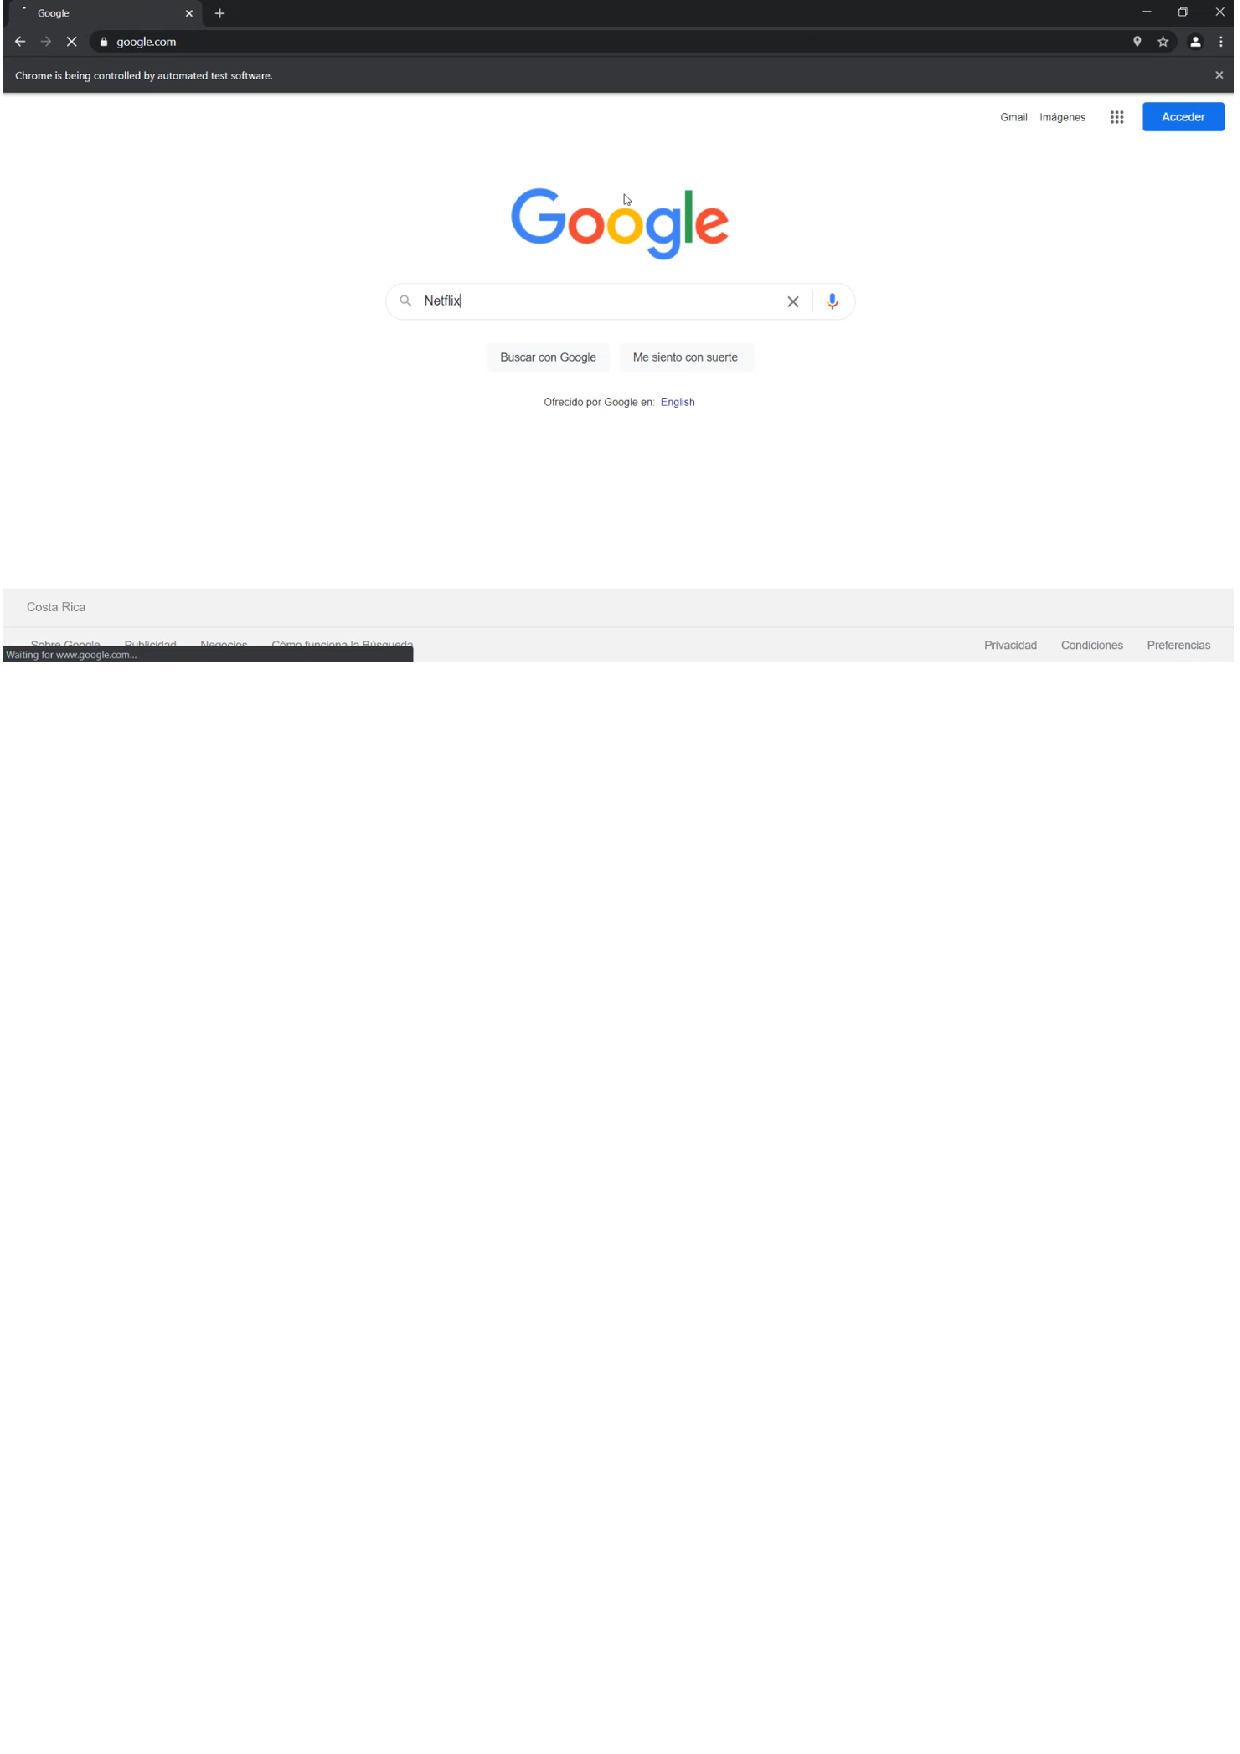
\includegraphics[scale=0.47]{imagenes/5buscanetflix.pdf}
\caption{Escribe en el buscador lo deseado}
\end{figure}

\begin{figure}[H]
\centering
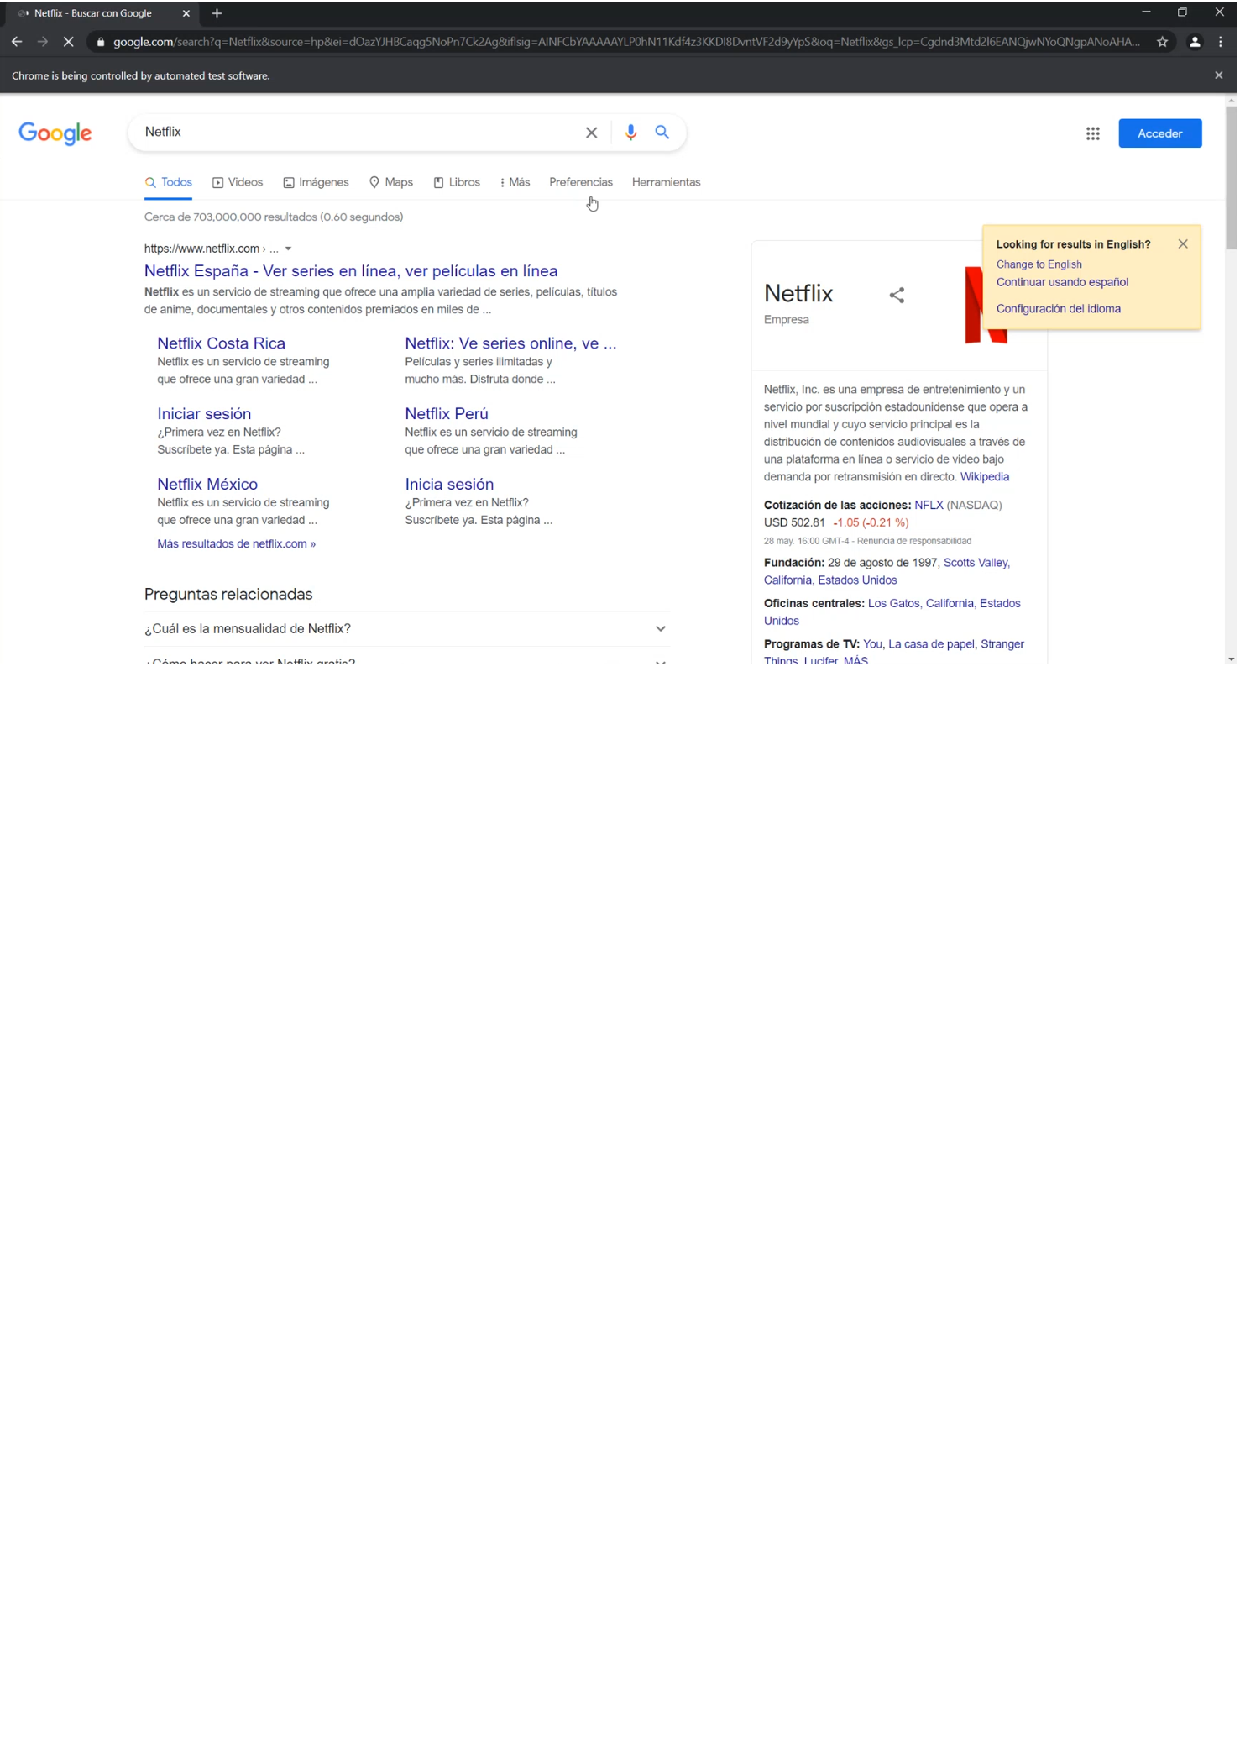
\includegraphics[scale=0.47]{imagenes/6clicknetflixcostarica.pdf}
\caption{Da click en la pagina deseada}
\end{figure}

\begin{figure}[H]
\centering
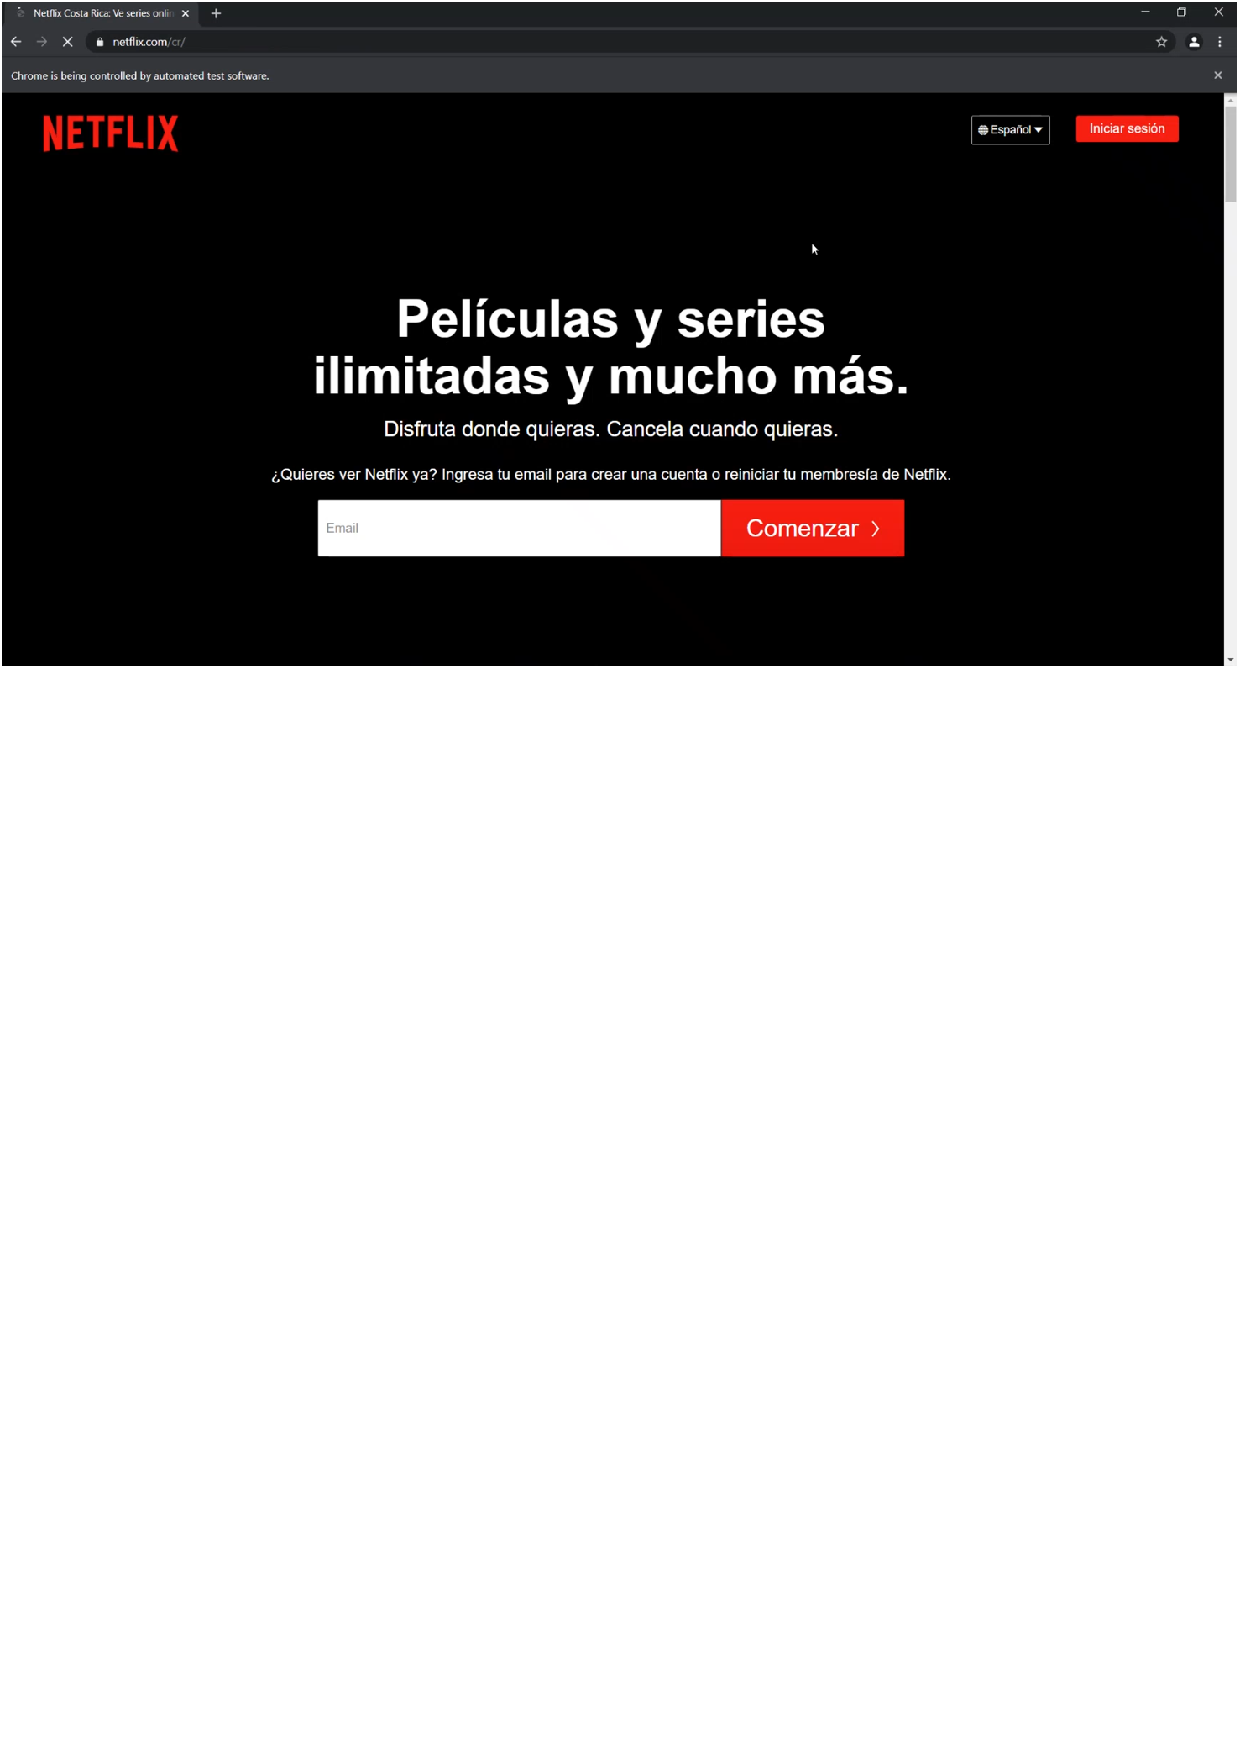
\includegraphics[scale=0.47]{imagenes/7abrelapaginayconfirmanombre.pdf}
\caption{Abre la pagina y comprueba que el titulo concuerde}
\end{figure}

Si la prueba falla, se muestra como un error normal y se indica el porque del fallo, en esta ocasión el titulo de la pagina no coincide con el que se estipula en el script.

\begin{figure}[H]
\centering
\includegraphics[scale=0.47]{imagenes/8testfail.pdf}
\caption{Test cuando falla}
\end{figure}

Cuando el test pasa, este genera un reporte con la información de la prueba. Dentro de la información esta la duración del test, si este pasa y a la hora en la que inicia.

\begin{figure}[H]
\centering
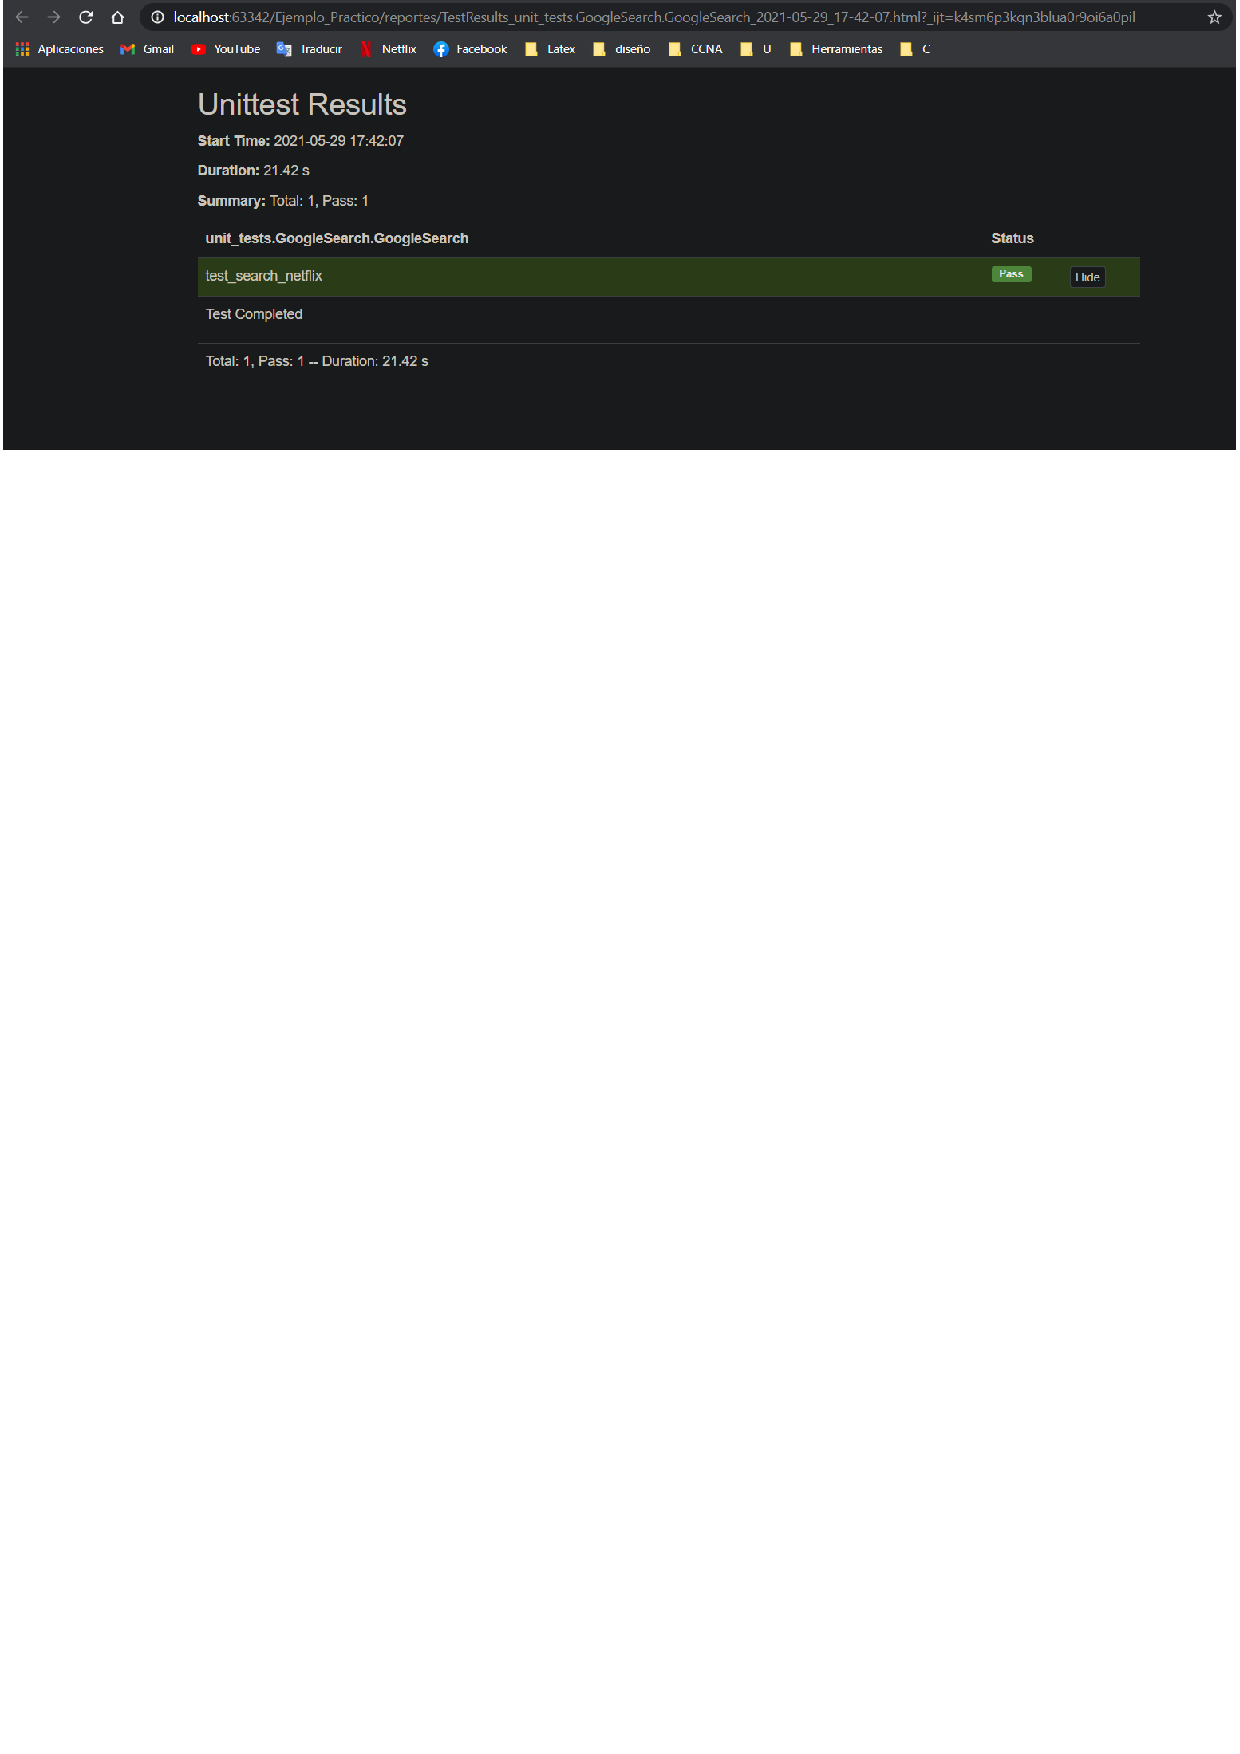
\includegraphics[scale=0.47]{imagenes/11testecompleto.pdf}
\caption{Test cuando pasa}
\end{figure}


\subsection{Prueba de regresión utilizando Selenium IDE}

Para poder utilizar esta opción, lo primero que se deber realizar es la descarga del IDE de Selenium, esta es una extension de Google Chrome.

\begin{figure}[H]
\centering
\includegraphics[scale=0.47]{imagenes/12SeleniumIDE.pdf}
\caption{Selenium IDE}
\end{figure}

Esta herramienta permite realizar pruebas de regresión  a paginas web sin tener que escribir código. En este ejemplo se probará que se pueda ingresar a la pagina de Facebook de Netflix. 

Este IDE registra las interacciones con sitios web para ayudar a generar y mantener la automatización del sitio, realizar pruebas y eliminar la necesidad de realizar tomas repetitivas manualmente.

La siguiente imagen es de la linea de comandos que debe realizar el test, cuando alguno de estos falla se pone en color rojo la linea que fallo.

\begin{figure}[H]
\centering
\includegraphics[scale=0.47]{imagenes/13COMANDOS.pdf}
\caption{Linea de comandos}
\end{figure}

\begin{figure}[H]
\centering
\includegraphics[scale=0.47]{imagenes/14seleniumfail.pdf}
\caption{Error en la linea de comandos}
\end{figure}

El IDE muestra cuales comandos logra completar y cuales no, los muestra conforme lo va realizando. En este ejemplo el tiempo de espera fue muy largo y no se pudo encontrar la pagina de Netflix - Home | Facebook.

\begin{figure}[H]
\centering
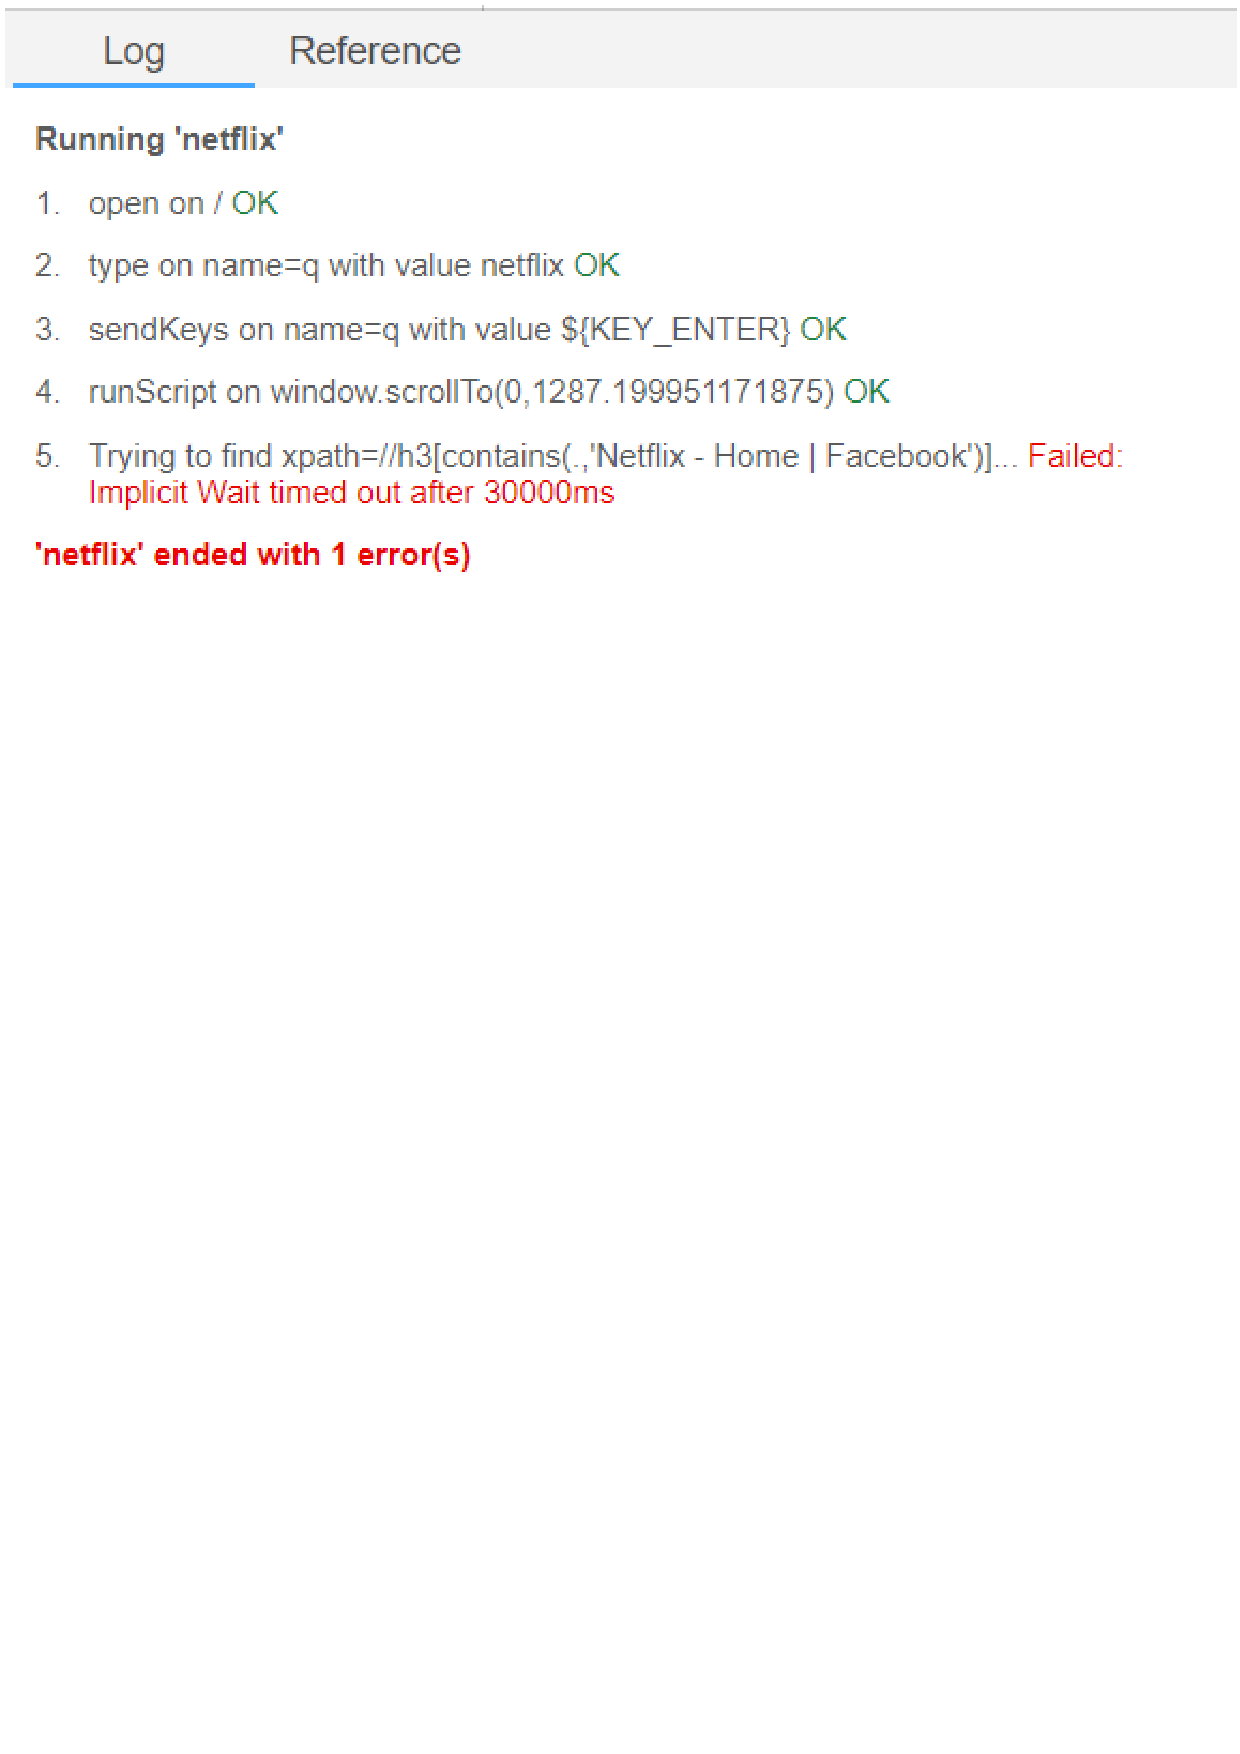
\includegraphics[scale=0.47]{imagenes/15Running.pdf}
\caption{Corrida en curso}
\end{figure}

Ejemplo de cuando el test logra completar todos los comandos establecidos.

\begin{figure}[H]
\centering
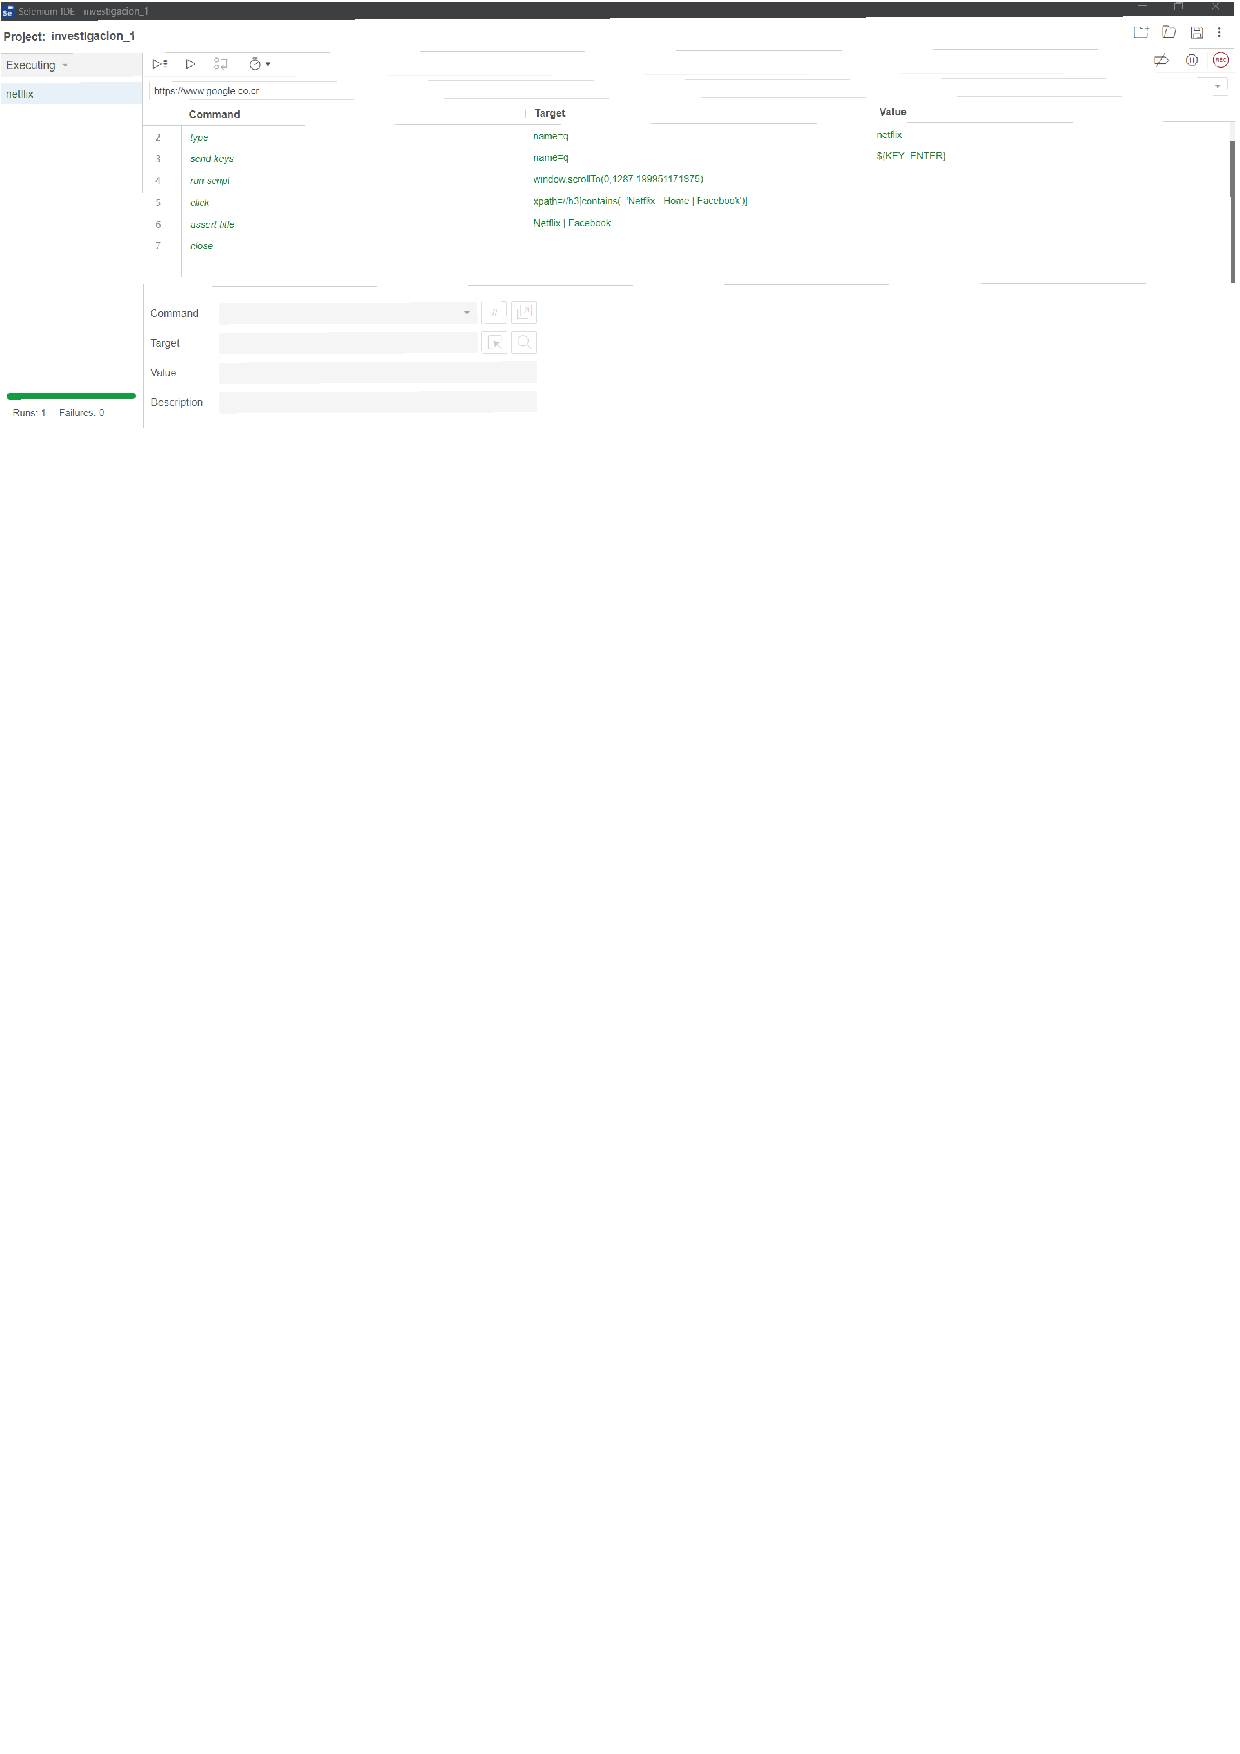
\includegraphics[scale=0.47]{imagenes/16seleniumpass.pdf}
\caption{Test cuando pasa}
\end{figure}

\begin{figure}[H]
\centering
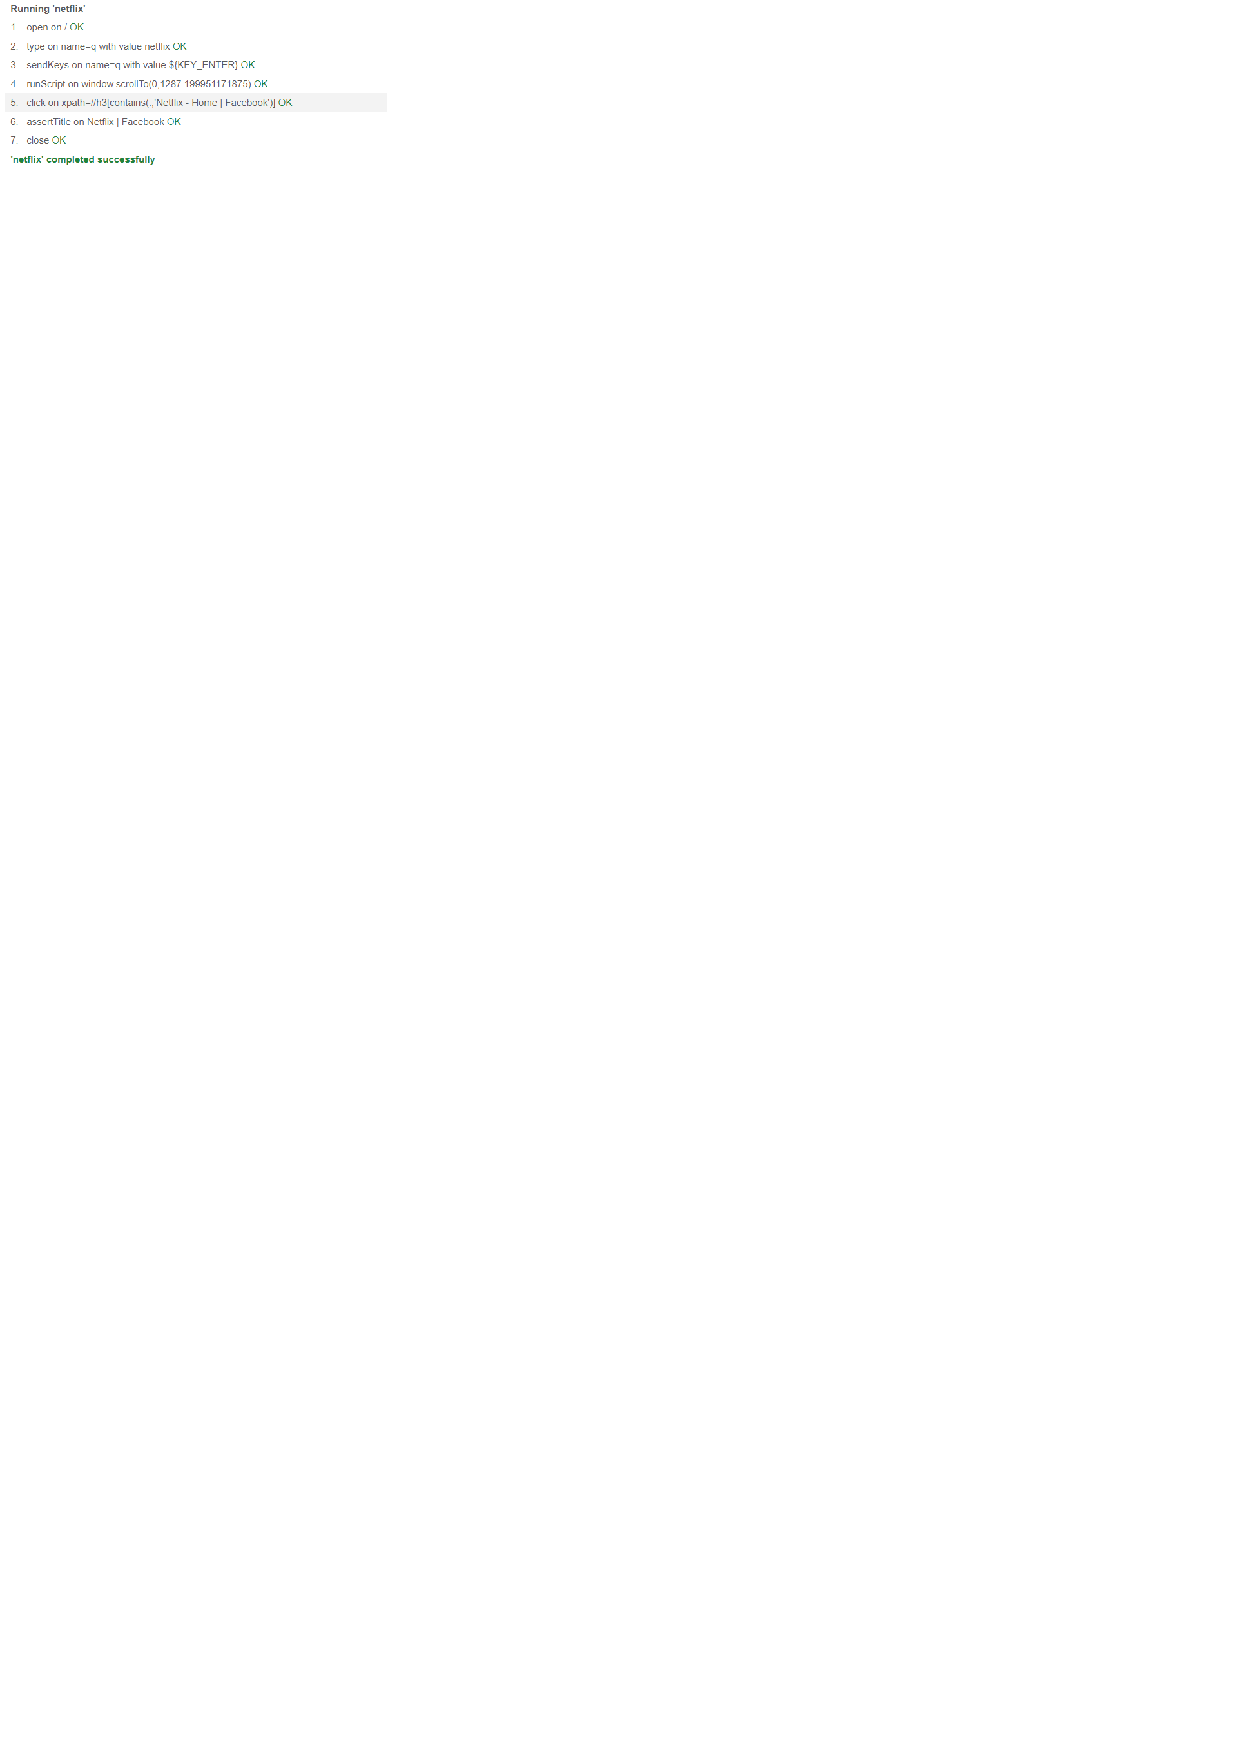
\includegraphics[scale=1.4]{imagenes/17runningpass.pdf}
\caption{Corrida en curso cuando pasa}
\end{figure}

El IDE lo que hace es grabar lo que se realiza en la pagina web esto lo convierte en comandos que posteriormente realiza automaticamente.


\begin{figure}[H]
\centering
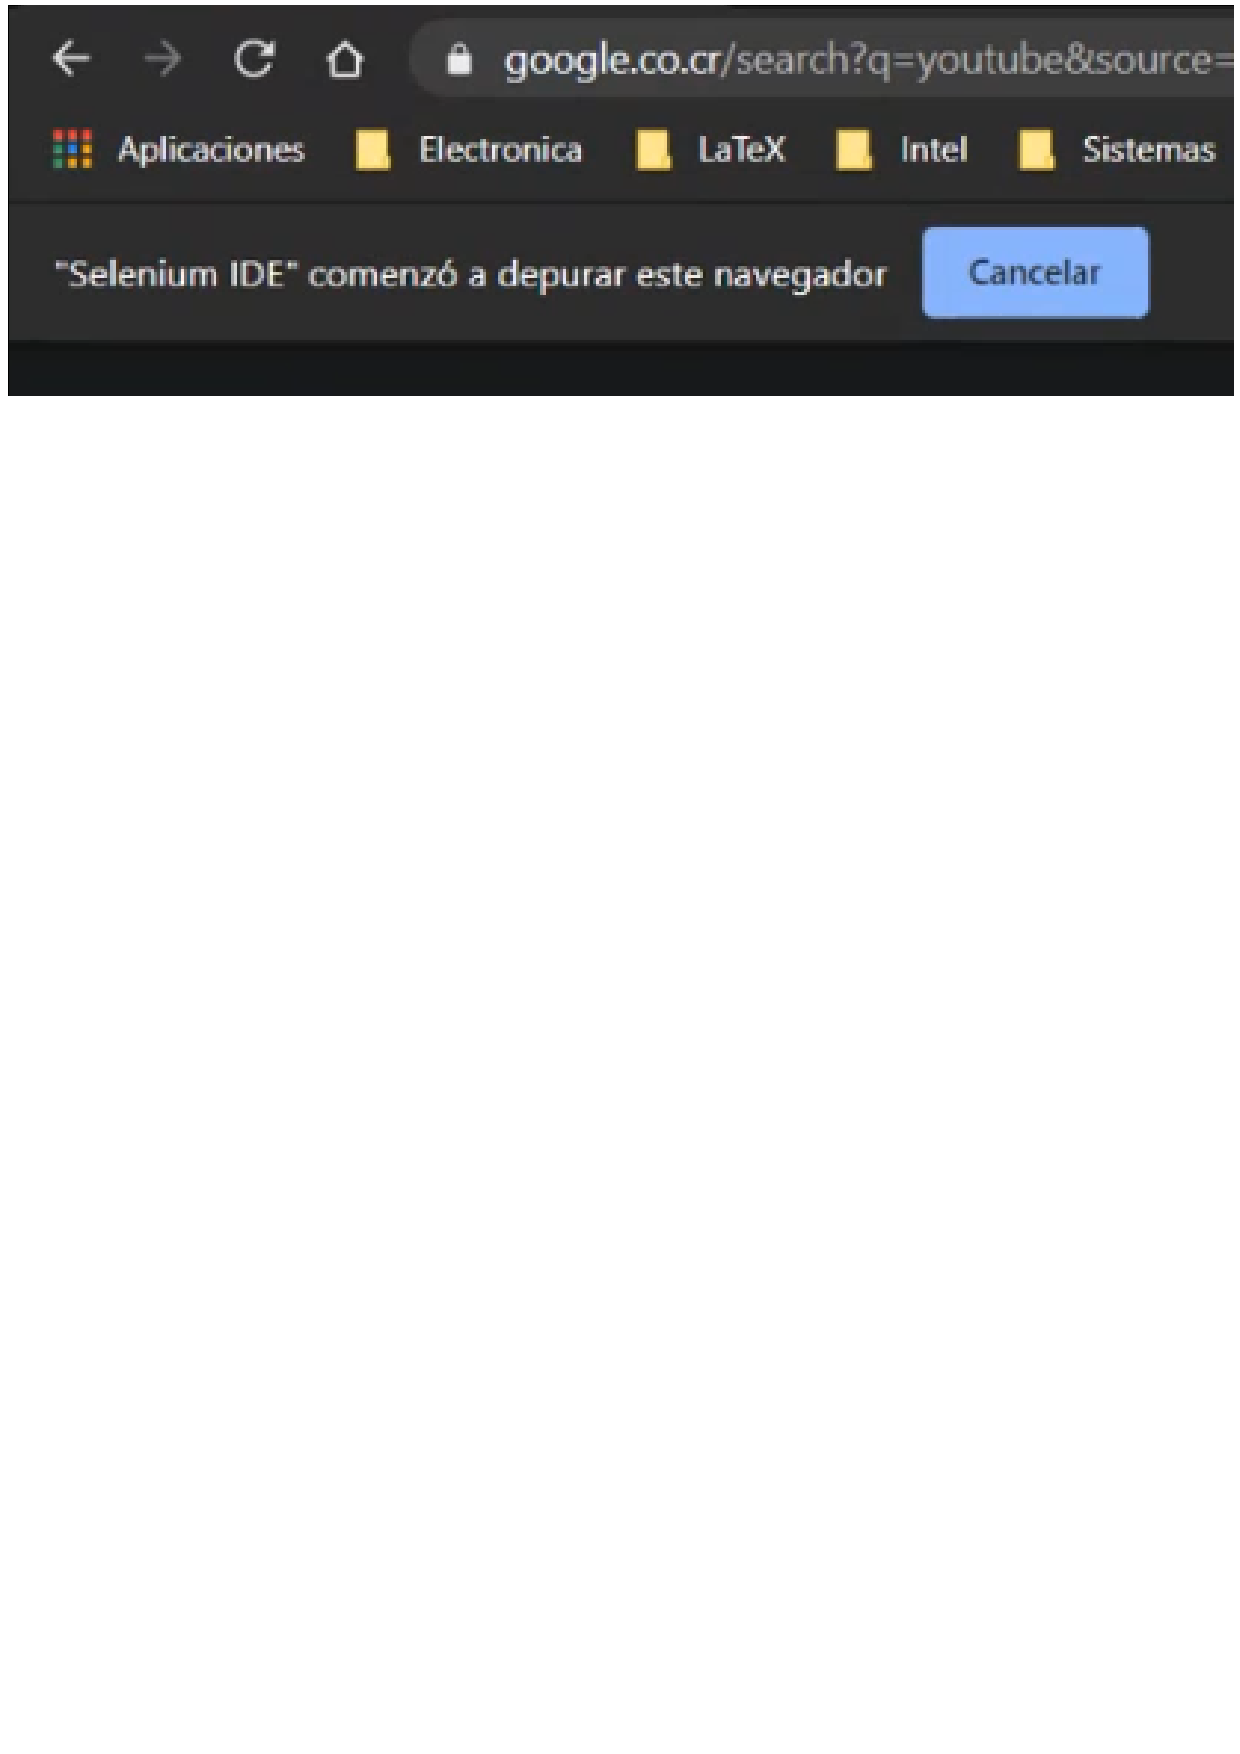
\includegraphics[scale=0.47]{imagenes/20.pdf}
\caption{Selenium IDE corriendo el test automáticamente}
\end{figure}


Lo primero que se debe realizar es especificarle al IDE cual pagina es la que debe abrir para comenzar el test. El espacio marcado con el color amarillo es donde se debe introducir el URL.

\begin{figure}[H]
\centering

\includegraphics[scale=0.47]{imagenes/18.pdf}
\caption{URL}
\end{figure}

Posterior a introducir el URL se debe comenzar a grabar para esto se debe dar click en el boton REC.

\begin{figure}[H]
\centering

\includegraphics[scale=0.47]{imagenes/19.1.pdf}
\caption{Botón de grabación}
\end{figure}

Para finalizar la grabación se pulsa el boton que esta  a la par del de grabar, pausar.

\begin{figure}[H]
\centering

\includegraphics[scale=0.47]{imagenes/19pausargrabacion.pdf}
\caption{Botón para pausar la grabación}
\end{figure}



Y de esa manera queda listo el test para correrlo. Esta es una opción interesante para las personas que no sepan programar.

%\section{Conclusiones}



\normalsize

\begin{thebibliography}{}
\bibitem{Alexynior} \textsc{Alexynior} (2019). \textit{¿Qué es una prueba de regresión?.} \url{https://adictec.com/que-son-pruebas-de-regresion/}\\

\bibitem{QAtesting} \textsc{The QA Testing Channel.} (2018). \textit{Pruebas de Regresión en 1 Minuto.} \url{https://www.youtube.com/watch?v=OEcIXnU6EQw} \\


\bibitem{INTERWARE} \textsc{INTERWARE} (2018). \textit{IMPORTANCIA DE REALIZAR REGRESSION TESTING.} \url{https://www.interware.com.mx/blog/importancia-de-realizar-pruebas-de-regresi\%C3\%B3n\#:\~:text=Se\%20dice\%20que\%20una\%20regresi\%C3\%B3n,que\%20todo\%20sigue\%20funcionando\%20bien.} \\

\bibitem{Isaac_Alvarez_Diz} \textsc{Isaac Álvarez Diz} (2018). \textit{¿Por qué un test de Regresión?} \url{https://qanewsblog.com/2018/01/22/por-que-un-test-de-regresion/} \\


\bibitem{Nerio_Rodriguez} \textsc{Nerio Rodriguez} (2017). \textit{TestingBaires - Generar Script con Selenium IDE} \url{https://www.youtube.com/watch?v=_yoAoZuKF78&list=PL-a9_OKTG4ShuvHjf3EVFYERnSf915K7G&index=3} \\

\bibitem{QA_Madness1} \textsc{QA Madness} (2021). \textit{Top-5 Tools for Regression Testing} \url{https://www.youtube.com/watch?v=HZvqfuADX8g} \\

\bibitem{QA_Madness2} \textsc{QA Madness} (2021). \textit{Regression testing – What, Why, When, and How to Run It?} \url{https://www.youtube.com/watch?v=AWX6WvYktwk} \\

\bibitem{Raghav_Pal} \textsc{Automation Step by Step - Raghav Pal} (2021). \textit{Selenium Python Small Sample Project 1 | Unit Test, HTML Reports} \url{https://www.youtube.com/watch?v=H9HUVSA_78U} \\

\bibitem{TestingWhiz} \textsc{TestingWhiz} (2020). \textit{General Information} \url{https://www.testing-whiz.com/user-manual} \\

\bibitem{Sahi Pro} \textsc{It'll take you more time to browse this website than to automate your test scripts using Sahi Pro} (2021). \url{https://www.sahipro.com/} \\

\bibitem{Avantica} \textsc{Adriana Chavarria} (2018). \textit{Pruebas de Regresión: 6 Recomendaciones para una buena planificación} \url{http://www.avantica.com/es/blog/pruebas-de-regresion-6-recomendaciones} \\

\bibitem{} \textsc{Manuel Cillero} (2021). \textit{Pruebas de Regresión} \url{https://manuel.cillero.es/doc/metodologia/metrica-3/tecnicas/pruebas/regresion/} \\

\bibitem{QA:news} \textsc{ISAACALVAREZ8180} (2018). \textit{¿Por qué un test de Regresión?} \url{https://qanewsblog.com/2018/01/22/por-que-un-test-de-regresion/} \\




\end{thebibliography}


\end{document}